% !TEX program = xelatex
\documentclass{article}
\usepackage{ctex, fontenc}
\usepackage{xcolor} % 在latex中使用颜色
\usepackage{booktabs,tabularx,multicol} % 制作表格
\usepackage{framed} % 制作文本框
\usepackage{amsmath,amsthm,amssymb,amsfonts}    % 数学符号与字体
\usepackage{bm} % 提供 \bm 加粗命令

\usepackage{algorithm}
\usepackage{algpseudocode}

% \usepackage{hyperref}   % 添加超链接
% \hypersetup{hidelinks} 
\usepackage[colorlinks=true, linkcolor=blue, citecolor=blue]{hyperref} % 引入 hyperref 包并设置颜色

\usepackage[paper=a4paper,text={146.6mm,244.1mm},top= 27.5mm,left=31.7mm,head=6mm,headsep=6.5mm,foot=7.9mm]{geometry}

\newtheorem{example}{Example}

\usepackage{appendix}   % 附录环境
\usepackage{subfig,graphicx}    % 插入照片
\usepackage{float}      % 固定浮动体
\usepackage{lipsum,zhlipsum} %生成一些测试文本
\usepackage{multirow}
\usepackage{tikz}
\usepackage{physics}

%---------------优雅的插入MATLAB代码---------%
\usepackage{listings,matlab-prettifier} % MATLAB 美化包
\lstset{
        style=Matlab-editor,
        numbers      = left,
        numbersep    = 5pt,
        numberstyle  = \small\color{red},
        frame        = single,
        keepspaces   = true,
        tabsize      = 4,
}


%-------------标题-------------%
\title{硕士毕业论文开题报告}
\date{\today}
\author{张阳}

%-----------做一些设置-----------%
\numberwithin{equation}{section}    % 公式标号与section的编号挂钩
\punctstyle{kaiming}    % 调整标点符号大小

%------------自定义一些命令------------%
\newcommand{\upcite}[1]{\textsuperscript{\textsuperscript{\cite{1}}}}



%---------------高亮--------------%
\usepackage{soul}
\addtocounter{MaxMatrixCols}{10}



%-------------------------- BEGIN ---------------------------------%
\begin{document}
\maketitle
\tableofcontents
\newpage

\section{方程与离散格式}
\subsection{方程介绍}
本文研究的二维欧拉方程可写为守恒形式如下:
\begin{equation}
    \frac{\partial \mathbf{U}}{\partial t}
    + \frac{\partial \mathbf{F}(\mathbf{U})}{\partial x}
    + \frac{\partial \mathbf{G}(\mathbf{U})}{\partial y}
    = \mathbf{S}(\mathbf{U}),
\end{equation}
其中,守恒变量 $\mathbf{U}$、通量项 $\mathbf{F}(\mathbf{U})$ 和 $\mathbf{G}(\mathbf{U})$ 以及源项 $\mathbf{S}(\mathbf{U})$ 分别为:
\begin{equation}
\mathbf{U} = \begin{bmatrix}
\rho       \\
\rho v_{x} \\
\rho v_{y} \\
\rho e
\end{bmatrix}, \quad
\mathbf{F}(\mathbf{U}) = \begin{bmatrix}
\rho v_{x}       \\
\rho v_{x}^{2}+P \\
\rho v_{x} v_{y} \\
(\rho e+P) v_{x}
\end{bmatrix}, \quad
\mathbf{G}(\mathbf{U}) = \begin{bmatrix}
\rho v_{y}       \\
\rho v_{y} v_{x} \\
\rho v_{y}^{2}+P \\
(\rho e+P) v_{y}
\end{bmatrix}, \quad
\mathbf{S}(\mathbf{U}) = \begin{bmatrix}
0      \\
0      \\
\rho g \\
\rho v_{y} g
\end{bmatrix}.
\end{equation}
其中,$\rho$ 为密度,$v_x$ 和 $v_y$ 分别为 $x$ 和 $y$ 方向的速度分量,$e$ 为总能量密度,$P$ 为压力,$g$ 为重力加速度。

气体状态方程采用理想气体状态方程
\begin{equation}
    P = (\gamma - 1)\rho \left( e - \frac{1}{2}(v_x^2 + v_y^2) \right),
\end{equation}
其中 $\gamma$ 是气体的比热比(通常取 $1.4$)。


%-----------------------------------%

本文研究的二维欧拉方程具有如下守恒形式:
\begin{equation}
    \frac{\partial \mathbf{U}}{\partial t}
    + \frac{\partial \mathbf{F}(\mathbf{U})}{\partial x}
    + \frac{\partial \mathbf{G}(\mathbf{U})}{\partial y}
    = \mathbf{S}(\mathbf{U}),
\end{equation}
其中,$\mathbf{U}$ 表示守恒变量向量,$\mathbf{F}(\mathbf{U})$ 和 $\mathbf{G}(\mathbf{U})$ 分别为 $x$ 和 $y$ 方向的通量函数,$\mathbf{S}(\mathbf{U})$ 为源项。各变量具体形式如下所示:
\begin{equation}
\mathbf{U} = \begin{bmatrix}
\rho       \\
\rho v_{x} \\
\rho v_{y} \\
\rho e
\end{bmatrix}, \quad
\mathbf{F}(\mathbf{U}) = \begin{bmatrix}
\rho v_{x}       \\
\rho v_{x}^{2}+P \\
\rho v_{x} v_{y} \\
(\rho e+P) v_{x}
\end{bmatrix}, \quad
\mathbf{G}(\mathbf{U}) = \begin{bmatrix}
\rho v_{y}       \\
\rho v_{y} v_{x} \\
\rho v_{y}^{2}+P \\
(\rho e+P) v_{y}
\end{bmatrix}, \quad
\mathbf{S}(\mathbf{U}) = \begin{bmatrix}
0      \\
0      \\
\rho g \\
\rho v_{y} g
\end{bmatrix}.
\end{equation}

其中,$\rho$ 为密度,$v_x$ 和 $v_y$ 分别表示 $x$ 和 $y$ 方向的速度分量,$e$ 是总能量密度,$P$ 为压力,$g$ 表示重力加速度。

气体的状态方程采用理想气体状态方程形式:
\begin{equation}
    P = (\gamma - 1)\rho \left( e - \frac{1}{2}(v_x^2 + v_y^2) \right),
\end{equation}
其中 $\gamma$ 为比热比,通常取值为 $1.4$。


\subsection{特征分析}

左右特征向量为\cite{RN95}:
\begin{equation}
    L_{i j}^{x}(u)=\begin{bmatrix}
        \dfrac{B_{2}+\mu / c}{2} & -\dfrac{B_{1} \mu+1 / c}{2} & -\dfrac{B_{1} v}{2} & \dfrac{B_{1}}{2} \\
        v                        & 0                           & -1                  & 0                \\
        1-B_{2}                  & B_{1} \mu                   & B_{1} v             & -B_{1}           \\
        \dfrac{B_{2}-\mu / c}{2} & -\dfrac{B_{1} \mu-1 / c}{2} & -\dfrac{B_{1} v}{2} & \dfrac{B_{1}}{2}
    \end{bmatrix}
\end{equation}
\begin{equation}
    R_{i j}^{x}(u)=\begin{bmatrix}
        1       & 0  & 1                        & 1       \\
        \mu-c   & 0  & \mu                      & \mu+c   \\
        v       & -1 & v                        & v       \\
        H-c \mu & -v & \dfrac{\mu^{2}+v^{2}}{2} & H+c \mu
    \end{bmatrix}
\end{equation}

\begin{equation}
    L_{i j}^{y}(u)=\begin{bmatrix}
        \dfrac{B_{2}+v / c}{2} & -\dfrac{B_{1} \mu}{2} & -\dfrac{B_{1} v+1 / c}{2} & \dfrac{B_{1}}{2} \\
        -\mu                   & 1                     & 0                         & 0                \\
        1-B_{2}                & B_{1} \mu             & B_{1} v                   & -B_{1}           \\
        \dfrac{B_{2}-v / c}{2} & -\dfrac{B_{1} \mu}{2} & -\dfrac{B_{1} v-1 / c}{2} & \dfrac{B_{1}}{2}
    \end{bmatrix}
\end{equation}
\begin{equation}
    R_{i j}^{y}(u)=\begin{bmatrix}
        1     & 0   & 1                        & 1     \\
        \mu   & 1   & \mu                      & \mu   \\
        v-c   & 0   & v                        & v+c   \\
        H-c v & \mu & \dfrac{\mu^{2}+v^{2}}{2} & H+c v
    \end{bmatrix}
\end{equation}

where  $c=\sqrt{\gamma p / \rho}, B_{1}=(\gamma-1) / c^{2}, B_{2}=B_{1}\left(\mu^{2}+v^{2}\right) / 2$  and  $H=(E+p) / \rho$

%--------------------------------------------%
在数值模拟中,特征分析是理解双相流动现象及其数值离散策略的关键步骤之一。特征分析主要用于判断方程组的类型(如抛物型、双曲型或椭圆型),并为构造稳定、高精度的数值格式提供理论基础。在本设计所使用的质量守恒形式下的两相流动控制方程为:

\begin{equation}
    \frac{\partial \mathbf{U}}{\partial t} + \nabla \cdot \mathbf{F}(\mathbf{U}) = \mathbf{S}(\mathbf{U}),
\end{equation}

其中 $\mathbf{U}$ 是守恒变量向量,$\mathbf{F}(\mathbf{U})$ 表示通量项,$\mathbf{S}(\mathbf{U})$ 为源项。为便于特征分析,我们忽略源项,并将二维形式简化为一维形式:

\begin{equation}
    \frac{\partial \mathbf{U}}{\partial t} + \frac{\partial \mathbf{F}(\mathbf{U})}{\partial x} = 0.
\end{equation}

该形式为典型的一阶准线性双曲型方程组。为了进一步分析其数学性质,我们对其进行特征分解。令雅可比矩阵 $\mathbf{A} = \partial \mathbf{F} / \partial \mathbf{U}$,则上式可以写为:

\begin{equation}
    \frac{\partial \mathbf{U}}{\partial t} + \mathbf{A} \frac{\partial \mathbf{U}}{\partial x} = 0.
\end{equation}

特征分析的核心是求解雅可比矩阵 $\mathbf{A}$ 的特征值和特征向量。设 $\lambda_i$ 是 $\mathbf{A}$ 的特征值,$\mathbf{r}_i$ 是对应的右特征向量,则系统的解可以沿着特征方向传播。这一性质为数值格式的构造(如Riemann求解器、特征分裂方法、WENO格式)提供了基础。

以两相流动中的双流体模型为例,其守恒变量 $\mathbf{U}$ 可表示为:

\begin{equation}
    \mathbf{U} = \begin{bmatrix}
    \alpha_1 \rho_1 \\
    \alpha_2 \rho_2 \\
    \alpha_1 \rho_1 u_1 \\
    \alpha_2 \rho_2 u_2 \\
    \end{bmatrix},
\end{equation}

其中 $\alpha_k$ 为相 $k$ 的体积分数,$\rho_k$ 和 $u_k$ 分别表示相 $k$ 的密度和速度。在无相间滑移的近似下,即 $u_1 \approx u_2 = u$,上述变量可进一步简化为单速度模型,从而得到如下形式的通量函数:

\begin{equation}
\mathbf{F}(\mathbf{U}) = \begin{bmatrix}
\alpha_1 \rho_1 u \\
\alpha_2 \rho_2 u \\
\alpha_1 \rho_1 u^2 + \alpha_1 p_1 \\
\alpha_2 \rho_2 u^2 + \alpha_2 p_2 \\
\end{bmatrix}.
\end{equation}

计算其雅可比矩阵 $\mathbf{A} = \partial \mathbf{F} / \partial \mathbf{U}$,即可求得系统的特征值。若所有特征值均为实数,且雅可比矩阵可对角化,则该方程组为双曲型系统。该性质意味着扰动以有限速度沿着特征线传播,这正是显式高精度格式(如TENO、WENO等)能够有效捕捉激波和界面变化的理论基础。

此外,特征分析还可用于判断系统中的波动类型。例如,在两相流中,不同的特征值可对应于压缩波、接触不连续面或相界面传播速度,这对于构造鲁棒的界面追踪方法(如THINC、VOF等)至关重要。

综上所述,特征分析不仅有助于理解两相流控制方程的数学性质,还为数值方法的设计与稳定性分析提供了有力支持。在后续的数值求解过程中,特征信息将在通量重构、界面捕捉以及边界处理等方面发挥重要作用。

\section{有限差分法离散格式}
有限差分法是一种经典且高效的数值离散方法,广泛应用于各类偏微分方程的求解中。在本设计所涉及的两相流动控制方程中,守恒型的形式适合采用有限差分方法进行高精度求解,特别是在处理激波、接触不连续面和相界面时,配合现代非振荡格式能够取得良好效果。

\subsection{空间离散}

空间离散的核心思想是用差分近似代替偏导数,从而将偏微分方程转化为差分方程。以一维守恒方程为例:

\begin{equation}
\frac{\partial \mathbf{U}}{\partial t} + \frac{\partial \mathbf{F}(\mathbf{U})}{\partial x} = 0,
\end{equation}

在有限差分框架下,我们以网格点 $\{x_i\}$ 上的守恒变量近似描述解的演化。将空间通量项离散为差分形式:

\begin{equation}
\frac{d \mathbf{U}_i}{d t} = -\frac{1}{\Delta x} \left( \hat{\mathbf{F}}_{i+1/2} - \hat{\mathbf{F}}_{i-1/2} \right),
\end{equation}

其中 $\hat{\mathbf{F}}_{i\pm 1/2}$ 为数值通量,通过对真实通量函数的重构或求解Riemann问题得到。在传统差分方法中,低阶中心差分或迎风差分易引起数值振荡或过度耗散,因此我们采用更高阶、更鲁棒的加权非振荡格式进行通量重构。

\paragraph{高阶非振荡通量重构}

为有效捕捉界面位置与流动不连续性,本文引入加权本征非振荡(TENO)格式进行空间重构。TENO格式在保持高阶精度的同时,具有良好的稳定性与非振荡性,其基本思想是利用多个局部插值子模板,通过平滑指标 $\beta_k$ 和权重函数构造加权通量:

\begin{equation}
\hat{\mathbf{F}}_{i+1/2}^{-} = \sum_{k=0}^{r-1} \omega_k q_k(x_{i+1/2}),
\end{equation}

其中 $q_k$ 是第 $k$ 个子模板上的通量插值函数,$\omega_k$ 是对应的权重,其大小依赖于局部平滑性指标 $\beta_k$。TENO 格式在光滑区间恢复高阶精度,在间断区自动退化为非振荡低阶格式,从而有效避免 Gibbs 现象。

\paragraph{界面捕捉方法——THINC函数}

在处理两相界面时,我们进一步引入THINC(Tangent of Hyperbola for INterface Capturing)函数对体积分数进行界面重构。THINC方法利用超曲线函数对不连续变量进行重构,表达如下:

\begin{equation}
\phi(x) = \frac{1}{2} \left(1 + \gamma \tanh\left( \beta \left( \frac{x - x_{i}}{\Delta x} - \tilde{x}_i \right) \right) \right),
\end{equation}

其中 $\gamma$ 表示界面方向,$\beta$ 控制过渡层厚度,$\tilde{x}_i$ 决定界面位置。该方法能够以极少的数值扩散精确保持界面形状,是处理多相流体体积分数演化的有力工具。

为更有效融合THINC和高阶格式,本文采用TENO-THINC混合格式,在平滑区使用TENO,在界面附近自动启用THINC策略,以提高界面保持能力和整体解的质量。

\subsection{时间离散}

在完成空间离散后,所得半离散系统为常微分方程形式:

\begin{equation}
\frac{d \mathbf{U}_i}{d t} = \mathcal{L}(\mathbf{U}),
\end{equation}

其中 $\mathcal{L}(\mathbf{U})$ 表示空间离散后的通量项差分。我们采用强稳定保持(SSP)型Runge-Kutta方法进行时间推进。以三阶显式SSP-RK方法为例,其格式如下:

\begin{align}
\mathbf{U}^{(1)} &= \mathbf{U}^n + \Delta t \, \mathcal{L}(\mathbf{U}^n), \\
\mathbf{U}^{(2)} &= \frac{3}{4} \mathbf{U}^n + \frac{1}{4} \left( \mathbf{U}^{(1)} + \Delta t \, \mathcal{L}(\mathbf{U}^{(1)}) \right), \\
\mathbf{U}^{n+1} &= \frac{1}{3} \mathbf{U}^n + \frac{2}{3} \left( \mathbf{U}^{(2)} + \Delta t \, \mathcal{L}(\mathbf{U}^{(2)}) \right).
\end{align}

该方法具有良好的稳定性,适用于包含间断或强梯度问题的数值模拟。

\subsection{小结}

通过空间上采用高阶TENO格式与界面专用的THINC重构相结合,时间上采用SSP-RK时间推进方案,本文建立了一个高精度、低耗散、界面保持能力强的有限差分离散格式。该方法能够准确模拟两相流动中的复杂界面演化、波传播和相互作用,为后续的数值模拟打下坚实基础。

\section{空间离散格式}
\subsection{WENO-JS格式}
\begin{figure}[!htbp]
    \centering
    \label{fig:}
    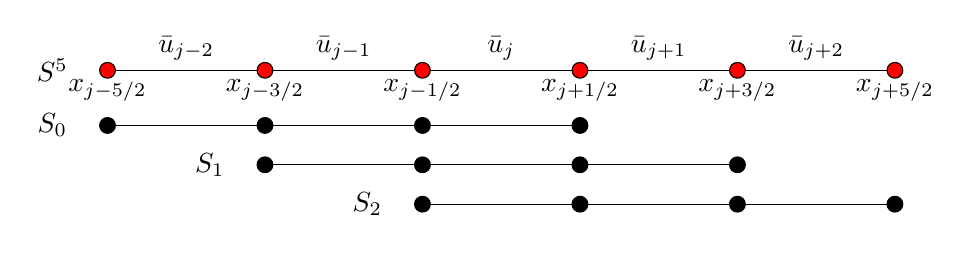
\begin{tikzpicture}
        \node[above] at (1,0) { $\bar{u}_{j-2}$ };
        \node[above] at (3,0) { $\bar{u}_{j-1}$ };
        \node[above] at (5,0) { $\bar{u}_{j}$ };
        \node[above] at (7,0) { $\bar{u}_{j+1}$ };
        \node[above] at (9,0) { $\bar{u}_{j+2}$ };
    
        \draw (0,0) -- (10,0);
        \foreach \x/\label in {0/{$x_{j-{5/2}}$},2/{$x_{j-{3/2}}$},4/{$x_{j-1/2}$},6/{$x_{j+1/2}$},8/{$x_{j+3/2}$},10/{$x_{j+5/2}$}} {
        \draw[fill=red] (\x,0) circle (0.1) node[below] {\label};
        }
        \node at (-0.7,0) { $S^5$ };
    
        \draw (0,-0.5-0.2) -- (6,-0.5-0.2);
        \foreach \x in {0,2,4,6} {
                \draw[fill=black] (\x,-0.5-0.2) circle (0.1) ;
            }
        \node at (-0.7,-0.5-0.2) { $S_0$ };
    
        \draw (2,-1-0.2) -- (8,-1-0.2);
        \foreach \x in {2,4,6,8} {
                \draw[fill=black] (\x,-1-0.2) circle (0.1) ;
            }
        \node at (1.3,-1-0.2) { $S_1$ };
    
        \draw (4,-1.5-0.2) -- (10,-1.5-0.2);
        \foreach \x in {4,6,8,10} {
                \draw[fill=black] (\x,-1.5-0.2) circle (0.1) ;
            }
        \node at (3.3,-1.5-0.2) { $S_2$ };
    
    \end{tikzpicture}
    \caption{}
\end{figure}

\begin{subequations}
    \begin{align}
        \hat{f}_{j+1/2}^0 &= \frac{1}{6}(2f_{j-2} - 7f_{j-1} + 11f_j),\\
        \hat{f}_{j+1/2}^1 &= \frac{1}{6}(-f_{j-1} + 5f_j + 2f_{j+1}),\\
        \hat{f}_{j+1/2}^2 &= \frac{1}{6}(2f_j + 5f_{j+1} - f_{j+2}).
    \end{align}
\end{subequations}
\begin{equation}
    \beta_k = \sum_{l=1}^2 \Delta x^{2l-1} \int_{x_{i-\frac{1}{2}}}^{x_{i+\frac{1}{2}}} \left( \frac{d^l}{dx^l} \hat{f}^k(x) \right)^2 dx.
\end{equation}
\begin{subequations}
    \begin{align}
    \beta_0 &= \frac{13}{12} (f_{i-2} - 2f_{i-1} + f_i)^2 + \frac{1}{4} (f_{i-2} - 4f_{i-1} + 3f_i)^2,\\
    \beta_1 &= \frac{13}{12} (f_{i-1} - 2f_i + f_{i+1})^2 + \frac{1}{4} (f_{i-1} - f_{i+1})^2,\\
    \beta_2 &= \frac{13}{12} (f_i - 2f_{i+1} + f_{i+2})^2 + \frac{1}{4} (3f_i - 4f_{i+1} + f_{i+2})^2.
    \end{align}
\end{subequations}
\begin{equation}
    d_0 = \frac{1}{10}, d_1 = \frac{6}{10}, d_2 = \frac{3}{10}.
\end{equation}
\begin{equation}
    \omega_k = \frac{\alpha_k}{\sum_{l=0}^2 \alpha_l}, \alpha_k = \frac{d_k}{(\beta_k + \epsilon)^p}. 
\end{equation}


\begin{equation}
    \hat{f}_{i\pm\frac{1}{2}} =\sum_{k=0}^2 \omega_k \hat{f}^k(x_{i\pm\frac{1}{2}})
\end{equation}



\subsection{WENO-Z格式}
\begin{equation}
    \omega_k^z = \frac{\mathbf{z}_k^z}{\sum_{l=0}^2\sigma_l^z}, \quad \mathbf{z}_k^z = \frac{d_k}{\beta_k^z} = d_k \left(1 + \frac{\tau_S}{\beta_k + \epsilon}\right), \quad k = 0,1,2,
\end{equation}

\subsection{边界条件}
% https://mp.weixin.qq.com/s/2bdiUI1BBu6gV7MrqQFHcQ

流体流动的边界条件是决定流体动力学行为的最重要因素之一,很久以来几乎在所有经典流体力学和润滑力学教科书或科技论文中,都有一个相同的重要假设:在固液界面上没有滑移,即固体表面上的流体分子和固体表面的相对运动速度为零。这就是经典的无滑移边界条件假设,该假设经过大量宏观意义上的实验验证,被广泛用于流体流动相关问题的分析、工程应用和实验研究等。首先需要明确的是,滑移/无滑移的概念是固体壁面边界与流体接触时,流体相对于壁面之间是否存在速度差?如果无相对速度,表示固壁为无滑移边界,其流体的速度取决于壁面的速度(静止/运动);如果存在相对速度,表示滑移边界。无滑移边界条件概念No-slip边界条件是在流体力学中常见的一种边界条件,它描述了流体与固体边界接触时的运动行为。该边界条件假设在流体与固体边界交界处,流体速度与固体表面相对运动速度为零,即流体在边界上附着并不滑动。这个假设是根据实际观察和实验得出的,特别适用于一些常见的流体行为,如空气或水与固体表面接触的情况。无滑移边界物理原理当流体与固体表面接触时,流体分子与固体表面之间存在分子间相互作用力,称为壁面粘附力。这种粘附力会使得流体分子在固体表面附近减速,并导致速度场在边界上附着,形成no-slip边界层。在no-slip边界层内,流体的速度梯度很大,因此流体颗粒在边界附近受到很强的黏性阻力,导致速度减小。随着流体颗粒离开边界越远,流体的速度逐渐恢复到远离边界处的自由流动速度。在no-slip边界层内,由于壁面粘附力的作用,流体的速度从静止的固体表面开始逐渐增加,直到达到自由流动速度。这种速度的变化率称为速度梯度。在no-slip边界层内,速度梯度非常大,即速度从静止到自由流动速度的变化很快。由于速度梯度的存在,no-slip边界层内的流体颗粒在与固体表面非常接近的地方会受到很强的黏性阻力作用。黏性阻力是由流体分子之间的相互作用力引起的,它使得流体颗粒在边界附近减速。因为黏性阻力的作用,no-slip边界层内的流体颗粒速度会减小。在接触固体表面的边界层内,流体的速度减小到接近零的程度。随着流体颗粒远离固体表面,黏性阻力逐渐减小,流体颗粒的速度逐渐恢复到远离边界的自由流动速度。在离开边界层的区域,流体的速度将接近自由流动速度,与未受壁面粘附力影响的远场流动速度相似。其中边界层的名义厚度表示为:当远离边界层的流体速度恢复至来流的99\%时,该位置距离边界的长度表示边界层厚度。在无滑移边界的情况下,根据固体壁面的运动情况可以进一步将边界条件划分为:无滑移静止壁面、无滑移运动壁面。无滑移静止壁面针对无滑移静止壁面边界,即固体表面是静止的, 速度为零。在数值模拟中,我们可以直接将边界上的流体速度设置为零,以满足no-slip边界条件。这意味着在静止壁面上,流体的速度与固体表面的速度相对运动速度为零,流体颗粒在边界附近停止运动。此时边界上流体的速度矢量为零,即法向速度和切向速度分量都等于零。无滑移运动壁面对于运动壁面,即固体表面具有一定的速度(假设是平移)。在这种情况下,我们需要根据固体表面的运动速度来设置边界上流体的速度。我们需要确保边界上流体的速度与固体表面速度的运动方向一致,并且速度大小等于固体表面速度的大小。例如方腔流的顶部就是无滑移运动壁面。在处理运动壁面时,需要特别注意边界速度的设置,以确保数值模拟得到准确的结果。特别是在涉及复杂的流动情况和边界运动时,边界条件的设置需要仔细考虑和验证。在商软fluent中对于无滑移运动壁面有三种处理方式:fluent无滑移运动壁面壁面相对于流体进行线性平动 Translational,由用户指定平动方向和速度大小。例如方腔流的顶部沿着  方向进行运动产生拖拽涡。如果是非线性平动,需要结合 Components 分量进行设置;如果是涉及旋转壁运动的边界,选择 Rotational 选项,定义旋转轴和旋转速度。该轴独立于相邻单元区域使用旋转轴,并且独立于任何其他壁旋转轴。对于三维问题,旋转轴是通过指定旋转轴原点并平行于从  到在旋转轴方向下指定的  点的矢量。对于二维问题,只需指定旋转轴原点;旋转轴是通过指定点的  方向矢量。对于二维轴对称问题,无需定义轴:旋转始终围绕  轴进行,原点位于 。滑移边界边界条件与无滑移边界对应的建模类型,则是滑移边界。滑移边界条件或速度偏移边界条件假定速度函数不连续,即流体与边界之间存在相对运动,因此存在滑移。速度函数在边界内有效达到边界速度的假设距离称为滑移长度 。Navier提出了线性滑移边界条件假设,该假设认为滑移速度与局部剪切率成正比:流体运动的速度边界模型分类示意图如图所示, 表示流体沿着固体表面  方向的切向流动速度;  是沿着界面法向方向坐标。(1)式被称为 滑移长度模型(Slip Length Model, SLM) ,由于  是常数,也被称为线性滑移长度模型。滑移长度只取决于流体和固体的配对,因此理论上可以通过实验确定。引入了克努森数,它允许对何时使用这两种条件中的哪一种进行粗略的数值近似。一般来说,在微流体学的大多数应用中,当处理特征长度尺度超过  的固体边界和不可压缩流体时,都可以使用无滑动边界条件。在高空、高超声速稀薄流动中,空气连续性假设条件部分失效,物面附近存在速度滑移情况。Maxwell 在1879年研究稀薄气体运动及其粘性阻力时,基于分子运动理论推导出了一阶泰勒展开近似滑移本构方程:式中  表示切向动量协调系数,其物理意义为气体分子在固体表面发生漫反射的分子数比例数。在实际工程中,常常假定固体表面足够粗糙,气体分子发生漫反射,于是通常情况下取值 。 是分子平均自由程,默认采用热力学参数进行计算:当  且  时,公式(2)和(1)是一样,大家后续在使用SLM时,并未实际区分流是液体还是气体。严格意义上来讲,公式(1)并没有从理论上证明适用于液体,只是Navier所作的假设。在实际流动过程中,流体在壁面附近是形成粘滞层,还是如线性滑移长度模型所述的在固体表面产生滑移,有待进一步研究。不知道目前该方面的定义是否进一步明确,可参考最新研究论文。

\subsection{边界条件}

求解模型控制方程,需要合理地选择边界条件。下面给出本文求解问题中所涉及的边界条件,包括:自由流入、自由流出、固壁反射边界条件。

\subsubsection{自由流入边界条件}
给定入口处流动状态,将物理量直接赋给边界点。
\subsubsection{自由流出边界条件}
出口为无反射边界条件。在出口边界处满足:

\begin{equation}
    \begin{cases} 
        \partial \rho / \partial n = 0 \\ 
        \partial u / \partial n = 0 \\ 
        \partial v / \partial n = 0 \\ 
        \partial p / \partial n = 0 
        \end{cases}
\end{equation}
其中,\(\partial / \partial n = \vec{n} \cdot \nabla\) 表示沿边界法线的方向导数。


\begin{equation}
    \begin{cases}
    \frac{\partial \rho}{\partial n} = 0 \
    \frac{\partial \mathbf{u}}{\partial n} = 0 \quad (\text{或} \ \frac{\partial u}{\partial n} = 0, \frac{\partial v}{\partial n} = 0) \
    \frac{\partial p}{\partial n} = 0
    \end{cases}
    \end{equation}
\subsubsection{固壁反射边界条件}
对于无粘、可压缩流场,固壁处采用滑移边界条件,即压力、密度、切向速度偏导数为零,法向速度为零:
\begin{equation}
    \begin{cases} 
        \partial \rho / \partial n = 0 \\ 
        \partial u / \partial n = 0 \\ 
        \partial v / \partial n = 0 \\ 
        v_n = 0 
        \end{cases}
\end{equation}


\begin{equation}
    \begin{cases}
    \frac{\partial \rho}{\partial n} = 0 \
    \frac{\partial p}{\partial n} = 0 \
    \frac{\partial u_\tau}{\partial n} = 0 \quad (\text{切向速度梯度为零}) \
    u_n = 0 \quad (\text{法向速度为零})
    \end{cases}
    \end{equation}
其中,\(\tau\) 代表切向,\(n\) 代表法向。
\section{时间离散格式-SSP-RK格式}
\begin{subequations}
    \begin{align}
        u^{(1)} &= u^n + \Delta t L \, (u^n)\\
        u^{(2)} &= \frac{3}{4}u^n + \frac{1}{4} \left[ u^{(1)} + \Delta t L \, (u^{(1)}) \right]\\
        u^{n+1} &= \frac{1}{3}u^n + \frac{2}{3} \left[ u^{(2)} + \Delta t L \, (u^{(2)}) \right]
    \end{align}
\end{subequations}
\begin{equation}
    \Delta t = \dfrac{CFL}{\dfrac{\lambda_{\max}}{\Delta x}+\dfrac{\lambda_{\max}}{\Delta y}  },
\end{equation}


\section{保正限制器}

\section{差分格式总结}
\begin{algorithm}[H]
    \caption{二维有限差分格式(特征分解 + 通量分裂)}
    \begin{algorithmic}[1]
    \State 初始化网格 $(x_i, y_j)$ 及时间步长 $\Delta t$
    \State 给定初始守恒变量 $U_{i,j}^0$
    \For{每个时间步 $n=0,1,\dots$}
        \For{每个网格点 $(i,j)$}
            \State 计算雅可比矩阵 $A = \partial F / \partial U$, $B = \partial G / \partial U$
            \State 对 $A$ 和 $B$ 进行特征分解,得左右特征向量 $L^x, R^x, L^y, R^y$ 及特征值 $\lambda^x, \lambda^y$
            \State 对通量进行分裂,例如 Lax-Friedrichs:
            \[
            F^{\pm} = \frac{1}{2}(F \pm \alpha^x U),\quad
            G^{\pm} = \frac{1}{2}(G \pm \alpha^y U)
            \]
            \State 将 $U$ 投影至特征空间:$W = L U$
            \State 对每个方向上的特征变量 $W$ 使用 WENO 插值构造左右状态 $W_{i\pm 1/2}^\mp$
            \State 还原通量:$F_{i+1/2} = R^x W_{i+1/2}$
            \State 使用有限差分格式更新通量导数:
            \[
            \left( \frac{\partial F}{\partial x} \right)_{i,j} \approx \frac{F_{i+1/2,j} - F_{i-1/2,j}}{\Delta x}
            \]
            \[
            \left( \frac{\partial G}{\partial y} \right)_{i,j} \approx \frac{G_{i,j+1/2} - G_{i,j-1/2}}{\Delta y}
            \]
            \State 更新守恒变量:
            \[
            U_{i,j}^{n+1} = U_{i,j}^n - \Delta t \left( \frac{\partial F}{\partial x} + \frac{\partial G}{\partial y} \right)
            \]
        \EndFor
    \EndFor
    \end{algorithmic}
    \end{algorithm}

\section{算例}
\begin{example}[二维欧拉方程光滑算例]{}{}
    光滑问题:初值为:
    \begin{equation}
        \begin{aligned}
            \rho(x,y,0) & = 1+0.2\sin(\pi(x+y)) \\
            u(x,y,0)    & = 0.7                 \\
            v(x,y,0)    & = 0.3                 \\
            p(x,y,0)    & = 1                   \\
        \end{aligned}
    \end{equation}
    周期边界条件

    准确解为:
    \begin{equation}
        \rho(x,y,t) = 1+0.2\sin(\pi(x+y-(u+v)t)),u=0.7,v=0.3,p=1
    \end{equation}
\end{example}
\begin{example}[二维欧拉方程黎曼问题]{}{}:
    % https://www.researchgate.net/publication/370612578_A_dissipation-dispersion_coupled_inequality_for_a_class_of_upwind_multi-resolution_WENO_schemes
    算例可参考:\cite{RN114}
    \begin{equation}
        (\rho, u, v, p)=\begin{cases}
            (0.138,1.206,1.206,0.029), & (x, y) \in[0,0.8) \times[0,0.8) \\
            (0.5323,1.206,0,0.3),      & (x, y) \in[0,0.8) \times[0.8,1] \\
            (0.5323,0,1.206,0.3),      & (x, y) \in[0.8,1] \times[0,0.8) \\
            (1.5,0,0,1.5),             & (x, y) \in[0.8,1] \times[0.8,1]
        \end{cases}
    \end{equation}
    $t_{end}=0.8$,网格为$400\times400$. 这个算例有时候会在两侧算出来几条等高线,例如\cite{ha2013modified,ha2016sixth,ha2024new},有时候不会,例如\cite{fleischmann2019numerical,liang2024new,jeong2022development}

    % \begin{figure}[H]%
    %     \centering
    %     \subfloat{
    %         \includegraphics[width=0.45\linewidth]{fig/黎曼问题图一.eps}
    %     }\quad
    %     \subfloat{
    %         \includegraphics[width=0.45\linewidth]{fig/黎曼问题图二.eps}
    %     }
    %     \caption{WENO-JS,M=200,等高线:0.2:0.05:1.7}
    % \end{figure}
\end{example}
\begin{example}[二维欧拉方程黎曼问题]{}{}
    二维黎曼问题\cite{RN13},初值为
    \begin{equation}
        (\rho, u, v, p)=\begin{cases}
            (0.8,0,0,1),      & (x, y) \in[0,1) \times[0,1) \\
            (1,0.7276,0,1),   & (x, y) \in[0,1) \times[1,2] \\
            (1,0,0.7276,1),   & (x, y) \in[1,2] \times[0,1) \\
            (0.5313,0,0,0.4), & (x, y) \in[1,2] \times[1,2]
        \end{cases}
    \end{equation}
    $p_1<p_2=p_3=p_4$.滑移边界条件.建议计算至$t=0.52$,网格为260*260.

    % \begin{figure}[H]%
    %     \centering
    %     \subfloat{
    %         \includegraphics[width=0.45\linewidth]{fig/黎曼算例2-1.png}
    %     }\quad
    %     \subfloat{
    %         \includegraphics[width=0.45\linewidth]{fig/黎曼算例2-2.png}
    %     }
    %     \caption{WENO-JS,M=10,等高线:linspace(0.56,1.67,30)}
    % \end{figure}
\end{example}
\begin{example}[二维欧拉方程Rayleigh-Taylor instability]
    \cite{liang2024new}
    The initial condition is
    \begin{equation}
        (\rho, u, v, p)=\left\{\begin{array}{ll}
            (2,0,-0.025 c \cos (8 \pi x), 1+2 y),   & 0 \leq y<1 / 2,      \\
            (1,0,-0.025 c \cos (8 \pi x), y+3 / 2), & 1 / 2 \leq y \leq 1,
        \end{array}\right.
    \end{equation}
    where  $c$  is the sound speed,  $c=\sqrt{\gamma \frac{p}{\rho}}$  with  $\gamma=\frac{5}{3}$ . The computational domain is  $[0,0.25] \times[0,1]$ . Reflecting boundary conditions are imposed on the left and right boundaries of the domain. Constant primitive variables  $(\rho, u, v, p)=(2,0,0,1)$  and  $(\rho, u, v, p)=(1,0,0,2.5)$  are set at the bottom and top boundaries, respectively.

    注意:这个算例需要增加源项,重力是向上的。



    % \begin{figure}[htp]
    %     \centering
    %     \label{fig:}
    %     \includegraphics[width=0.7\linewidth]{fig/RT_proble.png}
    %     \caption{}
    % \end{figure}

    算出不对称的结果也不用着急,参考文献里也有不对称的结果~\cite{shi2003resolution}


    这里有很多对RTI的分析
    Rahman, S. M., \& San, O. (2019). A Relaxation Filtering Approach for Two-Dimensional Rayleigh–Taylor Instability-Induced Flows. Fluids, 4(2). https://doi.org/10.3390/fluids4020078 

\end{example}



\clearpage
\bibliographystyle{unsrt}
\bibliography{ref}





\end{document}